\begin{frame}
\frametitle{Experiments - Paired Image Translation}
\framesubtitle{Baselines}
Training details:
\begin{itemize}
    \item 330MB of trainable parameters for unpaired models(LoRA weights, zero-conv layer, first conv layer of U-Net)
    \item Adam Optimizer with learning rate: 1e-6, batch size:8, $\lambda _{\text{idt}} = 1$, $\lambda _{\text{GAN}} = 0.5$
\end{itemize}
Datasets:
\begin{table}
    \centering
    \begin{tabular}{|c|c|c|c|}
        Task & Images Source & Images Target & Dataset \\
        \hline
        Horse $\leftrightarrow$ Zebra & 939 & 1177 & ImageNet \cite{5206848}\\
        Winter $\leftrightarrow$ Summer & 854 & 1273 & Flickr \cite{zhu2020unpaired} \\
        Day $\leftrightarrow$ Night & Day subset & Night subset & BDD100k \cite{yu2020bdd100k}\\
        Clear $\leftrightarrow$ Foggy & 12454 & 572 & BDD100k and DENSE \cite{bijelic2020seeing}
    \end{tabular}       
\end{table}
\end{frame}
\note{    
    \textbf{Erstens}: Vergleich mit diversen GAN- und Diffusion Modellen\\
    \textbf{Zweitens}: Analyse der verschiedenen Komponenten des Modells\\
    \textbf{Drittens}: Vergleich mit unpaired Methoden
    
    \begin{itemize}
        \item 330MB an trainierbaren Parametern, mit LoRA Gewichten, Zero-Conv Layer und erster Conv Layer des U-Net
        \item Adam Optimizer mit Lernrate: 1e-6, Batch-Size: 8, $\lambda _{\text{idt}} = 1$, $\lambda _{\text{GAN}} = 0.5$
        \item Horse $\leftrightarrow$ Zebra und Winter $\leftrightarrow$ Summer sind 286x286, hier wird zufällig auf 256x256 gecroppt. In Inference wird die Tranformation auf 256x256 durchgeführt.
        \item Day $\leftrightarrow$ Night und Clear $\leftrightarrow$ Foggy, hier wird auf 512x512 resized für training und Inference.
        \item Für Evaluation wird das zugehörige Validation-Set verwendet.4
    \end{itemize}

}

\begin{frame}
    \frametitle{Experiments - Paired Image Translation}
    \framesubtitle{Baselines}
    Evaluation Protocol:
    \begin{itemize}
        \item match data distribution of target domain $\rightarrow$ FID \cite{heusel2018gans}
        \item preserve input image structure in translated output $\rightarrow$ DINO \cite{tumanyan2022splicing}
        \item Inference runtime using a single NVIDIA RTX A6000 GPU
        \item human preceptual study
    \end{itemize}
\end{frame}
\note{
    Zwei wesentliche Ziele für Image Translation Modelle:\\
    \textbf{Erstens}: Die Verteilung der Ziel Domain möglichst gut matchen -> FID Score Frechet Inception Distance. Misst den Unterschied zwischen zwei Image sets (echt und fake). Basiert auf der Frechet Distance zwischen Zwei Wahrscheinlichkeitsverteilungen\\
    \textbf{Zweitens}: Die Struktur des Eingabebildes im übersetzten Bild erhalten -> DINO structural Distillation\\
    \begin{itemize}
        \item Ein niedriger FID Score zeigt einen guten Match zwichen der Verteilung der Ziel Domain und der generierten Bilder
        \item Ein niedriger DINO Score zeigt, dass die Struktur des Eingabebildes im übersetzten Bild erhalten bleibt
        \item niedriger FID und hoher DINO Score heißt, dass die Struktur des Eingabebildes im übersetzten Bild nicht erhalten bleibt
        \item hoher FID und niedriger DINO Score heißt, dass das Eingabebild kaum verändert wird -> Beide Scores betrachten
        \item zusätzlich wird die Inferenzzeit auf einer NVIDIA RTX A6000 GPU gemessen 
    \end{itemize}
}

% ---------- Comparison to Unpaired Methods ----------
\begin{frame}
    \frametitle{Experiments - Paired Image Translation}
    \framesubtitle{Comparison to Unpaired Methods}
    \begin{figure}
        \centering
        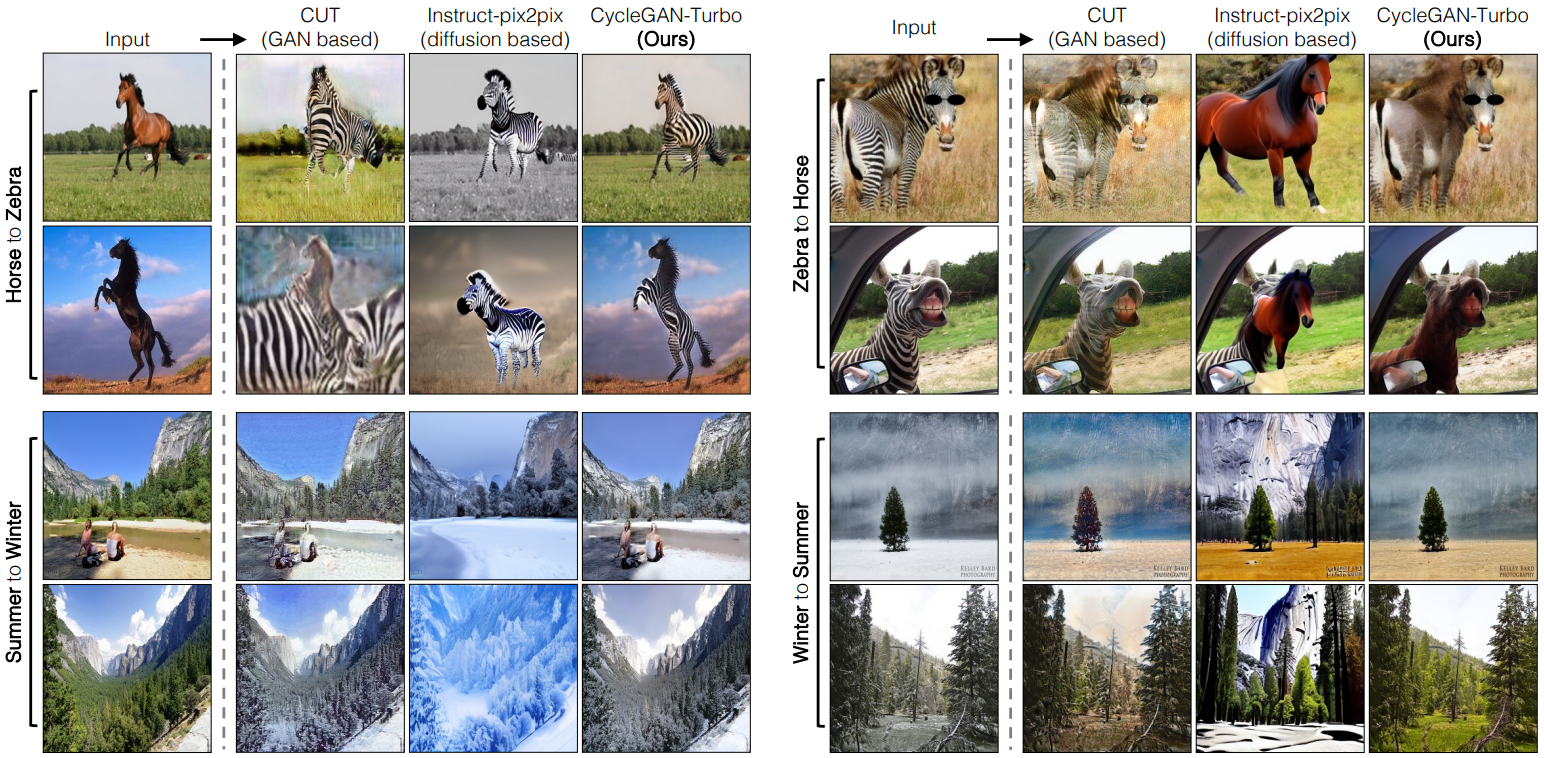
\includegraphics[width=0.85\linewidth]{images/horse_zebra.png}
        
    \end{figure}
\end{frame}
\note{
    Zuerst für die Tasks Horse $\rightarrow$ Zebra und Zebra $\rightarrow$ Horse und Winter $\rightarrow$ Summer und Summer $\rightarrow$ Winter
    \begin{itemize}
        \item Hier nur die Outputs für ein GAN-Modell und ein Diffusion-Modell. Für die Outputs der anderen Modelle für die Horse $\leftrightarrow$ Zebra Task verweise ich auf Anhang C im Paper
        \item Für die GAN-Modelle werden default Hyperparameter verwendet und auf allen Datensets für 100k Iterationen trainiert
    \end{itemize}
}




\begin{frame}
    \frametitle{Experiments - Paired Image Translation}
    \framesubtitle{Comparison to Unpaired Methods}
   
    \begin{table}
        \centering
    
     \vspace{-5pt}
        \resizebox{\linewidth}{!}{
        \begin{tabular}{l c cc cc cc cc}
            \toprule 
            \multirow{3}{*}{\textbf{Method}} 
            & \multirow{3}{*}{\textbf{\shortstack[c]{Infrence \\ time }}} 
            & \multicolumn{2}{c}{\textbf{Horse $\rightarrow$ Zebra} }
            & \multicolumn{2}{c}{\textbf{Zebra $\rightarrow$ Horse} }
            & \multicolumn{2}{c}{\textbf{Summer $\rightarrow$ Winter} }
            & \multicolumn{2}{c}{\textbf{Winter $\rightarrow$ Summer} }
            \\
    
            \cmidrule(lr){3-4} \cmidrule(lr){5-6} \cmidrule(lr){7-8} \cmidrule(lr){9-10} 
            &
            & \multirow{2}{*}{\shortstack[c]{FID $\downarrow$ }}  
            & \multirow{2}{*}{\shortstack[c]{DINO \\ Struct. $\downarrow$ }} 
    
            & \multirow{2}{*}{\shortstack[c]{FID $\downarrow$ }}  
            & \multirow{2}{*}{\shortstack[c]{DINO \\ Struct. $\downarrow$ }} 
    
            & \multirow{2}{*}{\shortstack[c]{FID $\downarrow$ }}  
            & \multirow{2}{*}{\shortstack[c]{DINO \\ Struct. $\downarrow$ }} 
    
            & \multirow{2}{*}{\shortstack[c]{FID $\downarrow$ }}  
            & \multirow{2}{*}{\shortstack[c]{DINO \\ Struct. $\downarrow$ }} 
            
            \\ \\
            \cmidrule(lr){1-10}
    
            CycleGAN \cite{zhu2020unpaired}  & 0.01s
            & 74.9 & 3.2 
            & 133.8 & 2.6
            & 62.9 & 2.6
            & 66.1 & 2.3 
            \\
            
            
            CUT \cite{park2020contrastive} & 0.01s
            & 43.9 & 6.6 
            & 186.7 & 2.5 
            & 72.1 & 2.1 
            & 68.5 & 2.1 \\
            
            \hdashline
    
            SDEdit \cite{meng2022sdedit} & 1.56s
            & 77.2 & 4.0
            & 198.5 & 4.6  
            & 66.1 & 2.1 
            & 76.9 & 2.1\\
            
            Plug\&Play \cite{tumanyan2022plugandplay} & 7.57s
            & 57.3 & 5.2  
            & 152.4 & 3.8 
            & 67.3 & 2.8 
            & 73.3 & 2.6\\
            
            Pix2Pix-Zero \cite{parmar2023zeroshot}  & 14.75s
            & 81.5 & 8.0
            & 147.4 & 7.8
            & 68.0 & 3.0
            & 93.4 & 4.3 \\
            
            Cycle-Diffusion \cite{cyclediffusion} & 3.72s
            & \textbf{38.6} & 6.0 
            & 132.5 & 5.8 
            & 64.1 & 3.6
            & 70.3 & 3.6 \\
    
            DDIB \cite{su2022dual} & 4.37s
            & 44.4 & 13.1  
            & 163.3 & 11.1 
            & 90.8 & 7.2
            & 88.9 & 6.8 \\
    
            InstructPix2Pix \cite{brooks2023instructpix2pix} & 3.86s
            & 51.0 & 6.8 
            & 141.5 & 7.0 
            & 68.3 & 3.7 
            & 85.6 & 4.4 \\
            \hdashline
    
            CycleGAN-Turbo & 0.13s
            & 41.0 & \textbf{2.1}
            & \textbf{127.5} & \textbf{1.8} 
            & \textbf{56.3} & \textbf{0.6} 
            & \textbf{60.7} & \textbf{0.6}\\
    
            \bottomrule 
        \end{tabular}
        }
        \vspace{-6pt}
    
        \label{tab:cmp_small_ds}
    \end{table}
\end{frame}
\note{
    \begin{itemize}
        \item Die Oberen 2 Zeilen zeigen die Ergebnisse der GAN-basierten Methoden, die unterste Zeile das Modell aus diesem Paper CycleGAN-Turbo. Die anderen Zeilen sind Diffusion-basierte Methoden
        \item Die erste spalte zeigt die Inferenzzeit auf einer NVIDIA RTX A6000 GPU. Die restlichen Spalten zeigen die FID und DINO Structural Distillation Scores die jeweiligen Tasks
        \item CycleGAN-Turbo erreicht die besten Ergebnisse in allen Tasks außer in der Horse $\rightarrow$ Zebra Task, wo es nur knapp hinter Cycle-Diffusion liegt, Cycle-Diffusion erzielt hier jedoch einen schlechten DINO Score und ist 28x Langsamer
    \end{itemize}

}




\begin{frame}
\frametitle{Experiments - Paired Image Translation}
\framesubtitle{Comparison to Unpaired Methods}
\begin{figure}
    \centering
    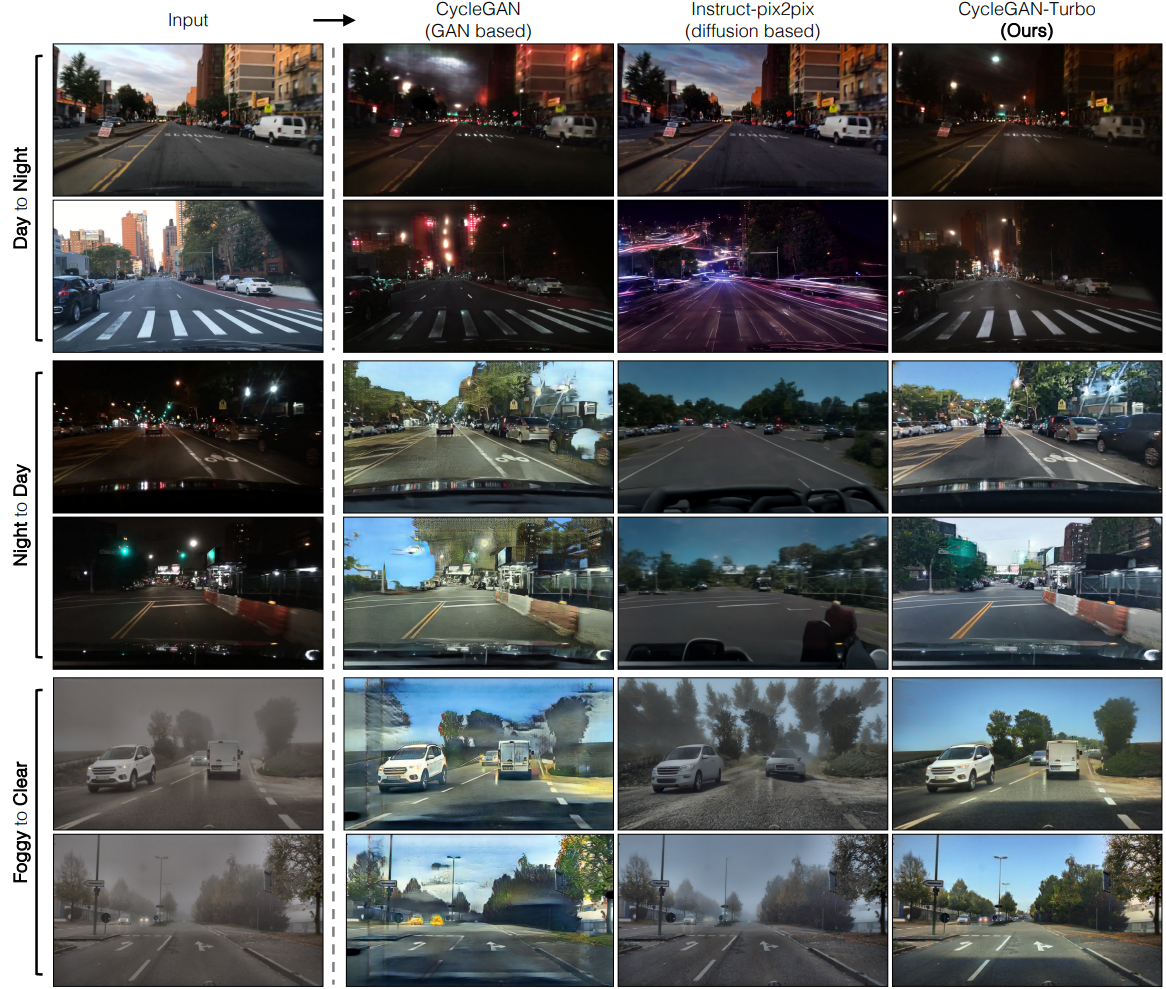
\includegraphics[width=0.5\linewidth]{images/day_night.png}
    
\end{figure}
\end{frame}
\note{   
    \begin{itemize}
        \item ähnliche Darstellung jetzt für die Tasks Day $\rightarrow$ Night und Night $\rightarrow$ Day und Foggy $\rightarrow$ Clear
        \item Von links nach rechts: Input, CycleGAN, InstructPix2Pix, CycleGAN-Turbo
    \end{itemize}

}





\begin{frame}
    \frametitle{Experiments - Paired Image Translation}
    \framesubtitle{Comparison to Unpaired Methods}

    \begin{table}
        \centering
    
        \resizebox{\linewidth}{!}{
        \begin{tabular}{l c cc cc cc cc}
            \toprule 
            \multirow{3}{*}{\textbf{Method}} 
            & \multirow{3}{*}{\textbf{\shortstack[c]{Infrence \\ time }}} 
            & \multicolumn{2}{c}{\textbf{Day $\rightarrow$ Night} }
            & \multicolumn{2}{c}{\textbf{Night $\rightarrow$ Day} }
            & \multicolumn{2}{c}{\textbf{Clear $\rightarrow$ Foggy} }
            & \multicolumn{2}{c}{\textbf{Foggy $\rightarrow$ Clear} }
            \\
    
            \cmidrule(lr){3-4} \cmidrule(lr){5-6} \cmidrule(lr){7-8} \cmidrule(lr){9-10} 
            &
            & \multirow{2}{*}{\shortstack[c]{FID $\downarrow$ }}  
            & \multirow{2}{*}{\shortstack[c]{DINO \\ Struct. $\downarrow$ }} 
    
            & \multirow{2}{*}{\shortstack[c]{FID $\downarrow$ }}  
            & \multirow{2}{*}{\shortstack[c]{DINO \\ Struct. $\downarrow$ }} 
    
            & \multirow{2}{*}{\shortstack[c]{FID $\downarrow$ }}  
            & \multirow{2}{*}{\shortstack[c]{DINO \\ Struct. $\downarrow$ }} 
    
            & \multirow{2}{*}{\shortstack[c]{FID $\downarrow$ }}  
            & \multirow{2}{*}{\shortstack[c]{DINO \\ Struct. $\downarrow$ }} 
            
            \\ \\
            \cmidrule(lr){1-10}
    
            CycleGAN \cite{zhu2020unpaired} & 0.02s
            & 36.3 & 3.6 
            & 92.3 & 4.9 
            & 153.3 & 3.6 
            & 177.3 & 3.9 
            \\
            
            CUT \cite{park2020contrastive} & 0.03s
            & 40.7 & 3.5 
            & 98.5 & 3.8
            & 152.6 & 3.4 
            & 163.9 & 4.8  \\
            
            \hdashline
    
            SDEdit \cite{meng2022sdedit} & 3.10s
            & 111.7 & 3.4 
            & 116.1 & 4.1 
            & 185.3 & 3.1
            & 209.8 & 4.7\\
    
            
            Plug\&Play \cite{tumanyan2022plugandplay} & 19.67s
            & 80.8 & 2.9 
            & 121.3 & \textbf{2.8} 
            & 179.6 & 3.6 
            & 193.5 & 3.5 \\
            
            Pix2Pix-Zero \cite{parmar2023zeroshot}  & 43.28s
            & 81.3 & 4.7 
            & 188.6 & 5.8
            & 209.3 & 5.5
            & 367.2 & 13.0
            \\
            
            Cycle-Diffusion \cite{cyclediffusion}  & 11.38s
            & 101.1 & 3.1 
            & 110.7 & 3.7 
            & 178.1 & 3.6 
            & 185.8 & 3.1\\
    
            DDIB \cite{su2022dual} & 11.93s
            & 172.6 & 9.1
            & 190.5 & 7.8 
            & 257.0 & 13.0 
            & 286.0 & 7.2  \\
    
            InstructPix2Pix \cite{brooks2023instructpix2pix} & 11.41s
            & 80.7 & \textbf{2.1} 
            & 89.4 & 6.2 
            & 170.8 & 7.6 
            & 233.9 & 4.8 
            \\
            \hdashline
    
            CycleGAN-Turbo & 0.29s
            & \textbf{31.3} & 3.0
            & \textbf{45.2} & 3.8 
            & \textbf{137.0} & \textbf{1.4}
            & \textbf{147.7} & \textbf{2.4} \\
    
            \bottomrule 
        \end{tabular}
        }
        \vspace{-18pt}
    
        \label{tab:cmp_driving_ds}
    \end{table}


\end{frame}
\note{
    \begin{itemize}
        \item Auch hier hat CycleGAN-Turbo die besten Ergebnisse in allen Tasks
        \item InstructPix2Pix und Plug\&Play haben zwar bessere DINO Scores, jedoch wesentlich schlechtere FID Scores
    \end{itemize}

}


% ---------- Ablation Study ----------
\begin{frame}
\frametitle{Experiments - Paired Image Translation}
\framesubtitle{Ablation Study}


    \begin{table}   
        \centering
        \resizebox{\linewidth}{!}{
        \begin{tabular}{l c c c | cc cc cc cc}
            \toprule 
            \multirow{3}{*}{\textbf{Method} }
            & \multirow{3}{*}{\shortstack[c]{\textbf{Input} \\ \textbf{Type} }}  
            & \multirow{3}{*}{\shortstack[c]{\textbf{Skip} }}  
            & \multirow{3}{*}{\shortstack[c]{\textbf{Pre} \\ \textbf{-trained} }}  
            & \multicolumn{2}{c}{\textbf{Horse $\rightarrow$ Zebra} }
            & \multicolumn{2}{c}{\textbf{Zebra $\rightarrow$ Horse} }
            \\
    
            \cmidrule(lr){5-6} \cmidrule(lr){7-8} \cmidrule(lr){9-10} \cmidrule(lr){11-12} 
    
            &&&& \multirow{2}{*}{\shortstack[c]{FID $\downarrow$ }}  
            & \multirow{2}{*}{\shortstack[c]{DINO \\ Struct. $\downarrow$ }} 
    
            & \multirow{2}{*}{\shortstack[c]{FID $\downarrow$ }}  
            & \multirow{2}{*}{\shortstack[c]{DINO \\ Struct. $\downarrow$ }} 
            
            \\ \\
            \cmidrule(lr){1-12}
            Conf. A & Direct Input & x & x
            & 128.6 (+214\%)  & 5.2 (+148\%)
            & 167.1 (+31\%)  & 4.6 (+156\%)
            \\
            
            Conf. B & ControlNet & x & \checkmark 
            & 41.2 (+0\%)  & 7.3 (+248\%)
            & \textbf{99.4 (-22\%)}  & 8.6 (+378\%)\\
    
            Conf. C & T2I-Adapter & x & \checkmark 
            & 55.4 (+35\%)  & 4.7 (+124\%)
            & 135.4 (+6\%) & 4.8 (+167\%)\\
            
            
            Conf. D & Direct Input & x & \checkmark
            & \textbf{40.1 (-2\%)}  & 4.4 (+110\%)
            & 116.2 (-9\%) & 3.0 (+67\%) \\
            
            
            \hdashline
            Ours & Direct Input & \checkmark & \checkmark
            & 41.0 & \textbf{2.1}
            & 127.5 & \textbf{1.8}  \\
    
            \bottomrule 
        \end{tabular}
        }
    \vspace{-10pt}
        \label{tab:ablation_study}
    \end{table}
\end{frame}
\note{
    \begin{itemize}
        \item Für diesen Vergleich mit anderen Tasks verweise auf Anhang A im Paper. Spoiler: Das Ergebniss ist vergleichbar
        \item Hier wird die Wichtigkeit der verschiedenen Komponenten des Modells untersucht
        \item Conf. A: Direkter Input, keine Pre-trained Gewichte, Gewichte random initialisiert, schlechteste Ergebnisse
        \item Conf. B, C, D nutzen verschieden Pre-trained Gewichte, Conf D hat unter denen die besten Ergebnisse
        \item Zu dieser Konfiguration werden dann Skip-Connections hinzugefügt, was die Ergebnisse nochmal verbessert
    \end{itemize}
}

\begin{frame}
    \frametitle{Experiments - unpaired Image Translation}
    \framesubtitle{Ablation Study}
    \begin{figure}
        \centering
        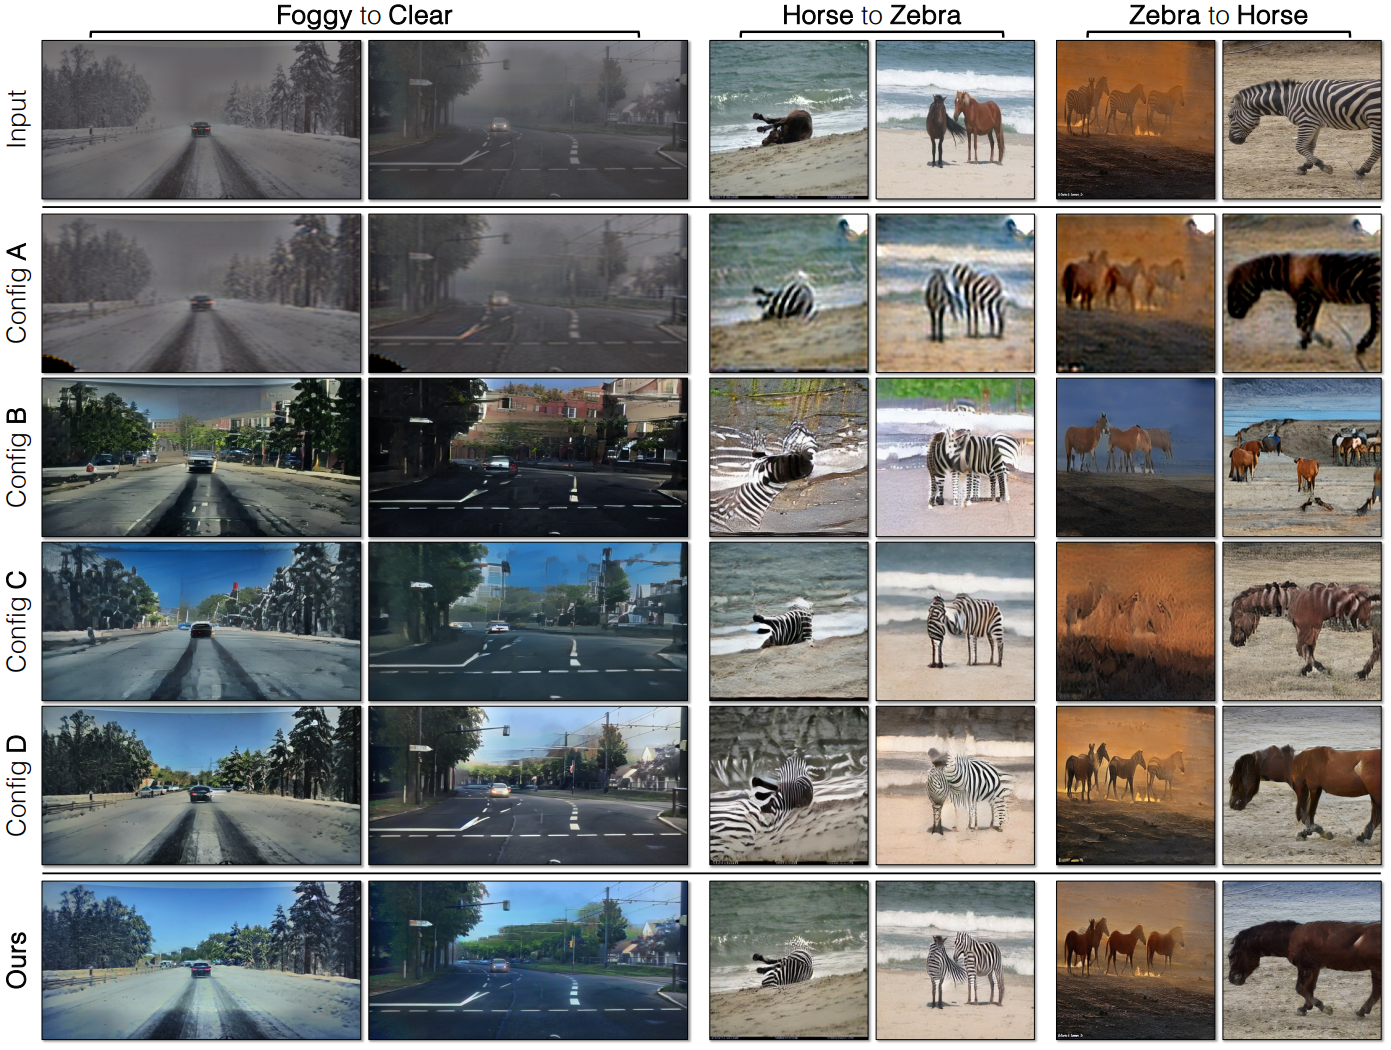
\includegraphics[width=0.55\linewidth]{images/ablation_images.png}
        
    \end{figure}
\end{frame}
\note{
    \begin{itemize}
        \item zu den jeweiligen Konfigurationen werden hier die Outputs für Horse $\rightarrow$ Zebra, Zebra $\rightarrow$ Horse und Foggy $\rightarrow$ Clear gezeigt
        \item Für die Outputs der anderen Taks verweise ich auf Anhang B im Paper
    \end{itemize}
}
% ---------- Extensions ----------
\begin{frame}
\frametitle{Experiments - Paired Image Translation}
\framesubtitle{Training Details}
\begin{block}{Loss function}
    \begin{align}
        \arg \underset{G}{\min} \mathcal{L}_{\text{rec}} + \lambda _{\text{clip}} \mathcal{L}_{\text{CLIP}} + \lambda_{\text{GAN}}\mathcal{L}_{\text{GAN}}
    \end{align}
\end{block}
with $\mathcal{L}_{\text{rec}}$ = L2-Norm + LPIPS, $\lambda_{\text{clip}} = 4$ and $\lambda_{\text{GAN}} = 0.4$
\end{frame}
\note{
    \begin{itemize}
        \item Hier wird die Loss-Funktion gezeigt, die für das Training verwendet wird
        \item $\mathcal{L}_{\text{rec}}$ Reconstruction Loss, die aus der L2-Norm und LPIPS besteht
        \item $\lambda_{\text{clip}}$ = 4
        \item $\lambda_{\text{GAN}}$ = 0.4
        \item LPIPS?
        \item CLIP?
    \end{itemize}
}

\begin{frame}
    \frametitle{Experiments - Paired Image Translation}
    \framesubtitle{Training Details}
    basiert auf Midjourney-Datensatz \footnote{https://huggingface.co/datasets/wanng/midjourney-v5-202304-clean}\\
        Edge-to-Image:
        \begin{itemize}
            \item Canny Edge Detector with random threshold
            \item Adam Optimizer with learning rate: 1e-5, batch size: 40, Steps: 7500
        \end{itemize}
        Sketch-to-Image:
        \begin{itemize}
            \item Synthetic sketches with multiple augmentations
            \item Initialized with Edge-to-Image model and fine-tuned for 5000 steps with same Optimizer
        \end{itemize}
\end{frame}
\note{
    \begin{itemize}
        \item Hier werden zwei Modelle trainiert, die auf dem Midjourney-Datensatz basieren
        \item Edge-to-Image: Hier werden mit dem Canny Edge Detector mit einem random Threshold Kanten erzeugt. \\Adam Optimizer mit Lernrate: 1e-5, Batch-Size: 40, 7500 Schritte
        \item Sketech-to-Image: Mit mehreren Augmentation werden aus den Bildern Sketches erzeugt.\\ Das Modell wird mit dem Edge-to-Image model initialisiert und dann nochmal für 5000 Schritte trainiert.
    \end{itemize}

}

\begin{frame}
    \frametitle{Experiments - Paired Image Translation}
    \framesubtitle{Comparison to Paired Methods}
    \begin{figure}
        \centering
        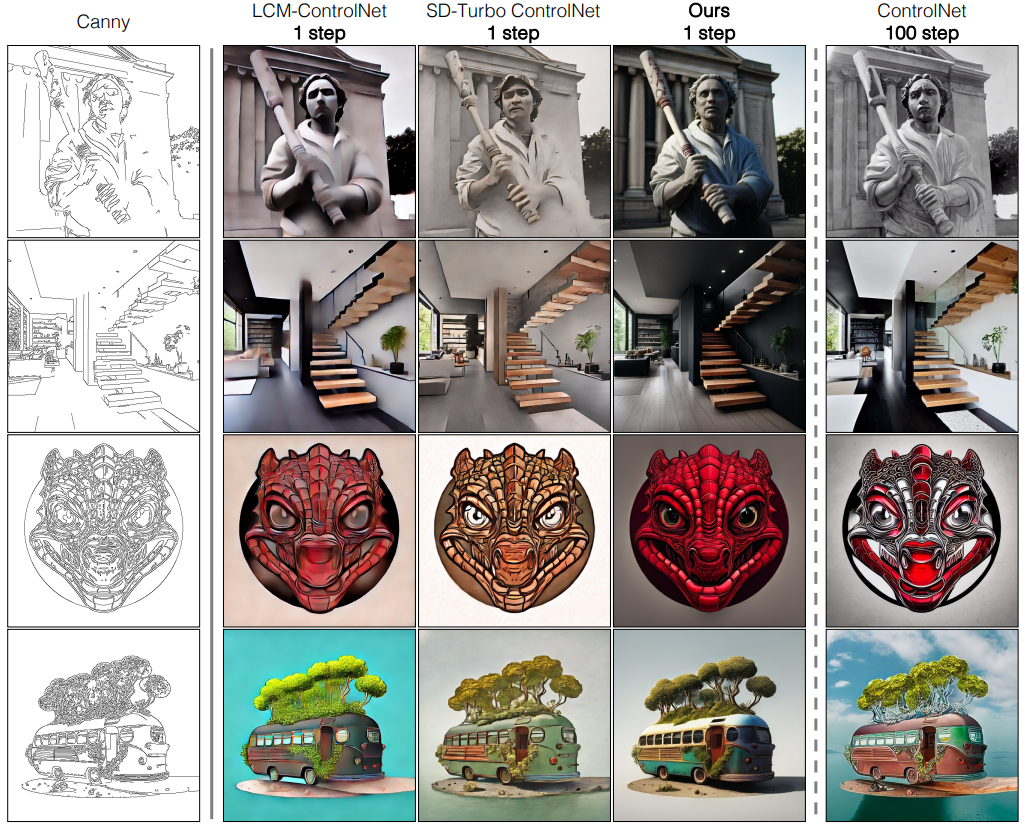
\includegraphics[width=0.5\linewidth]{images/unpaired_comp1.png}
        
    \end{figure}
\end{frame}
\note{
    \begin{itemize}
        \item Hier Edge-to-Image im Vergleich zu anderen Modellen
        \item Sichtbar mehr Realismus als die anderen Modelle
        \item Vergleichbarer Realismus zu ControlNet mit 100Schritten, obwohl das Edge-To-Image Modell 65x schneller ist
    \end{itemize}

}

\begin{frame}
    \frametitle{Experiments - Paired Image Translation}
    \framesubtitle{Comparison to Unpaired Methods}
    \begin{figure}
        \centering
        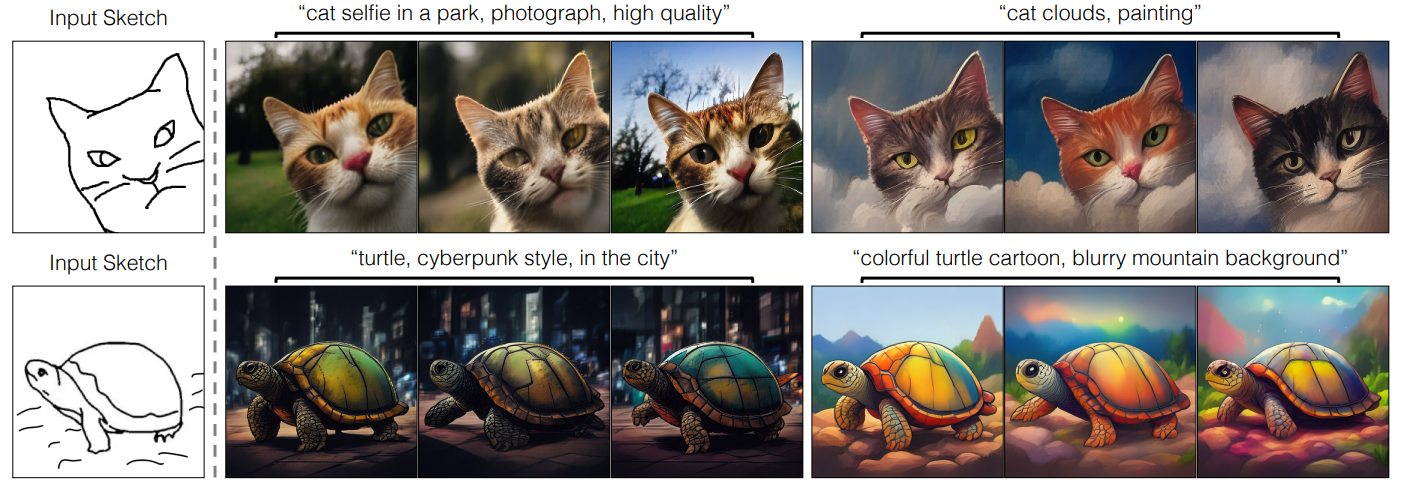
\includegraphics[width=1\linewidth]{images/unpaired_comp2.png}
            
    \end{figure}
\end{frame}
\note{
    \begin{itemize}
        \item Wie in der Methode beschrieben, ist es möglich mit dem selben Sketch und Prompt verschiedene Outputs zu generieren
    \end{itemize}
}
